\chapter{Cylindrical Simulations to Study the Effect of Beam Radius in Direct-Drive}



%###############################################################################################################################
%###############################################################################################################################
%###############################################################################################################################
\section{Introduction to Beam Radius in Direct-Drive Inertial Confinement Fusion}%
\label{sec:Res1_Beamrad_intro}

\begin{figure}[t!]
    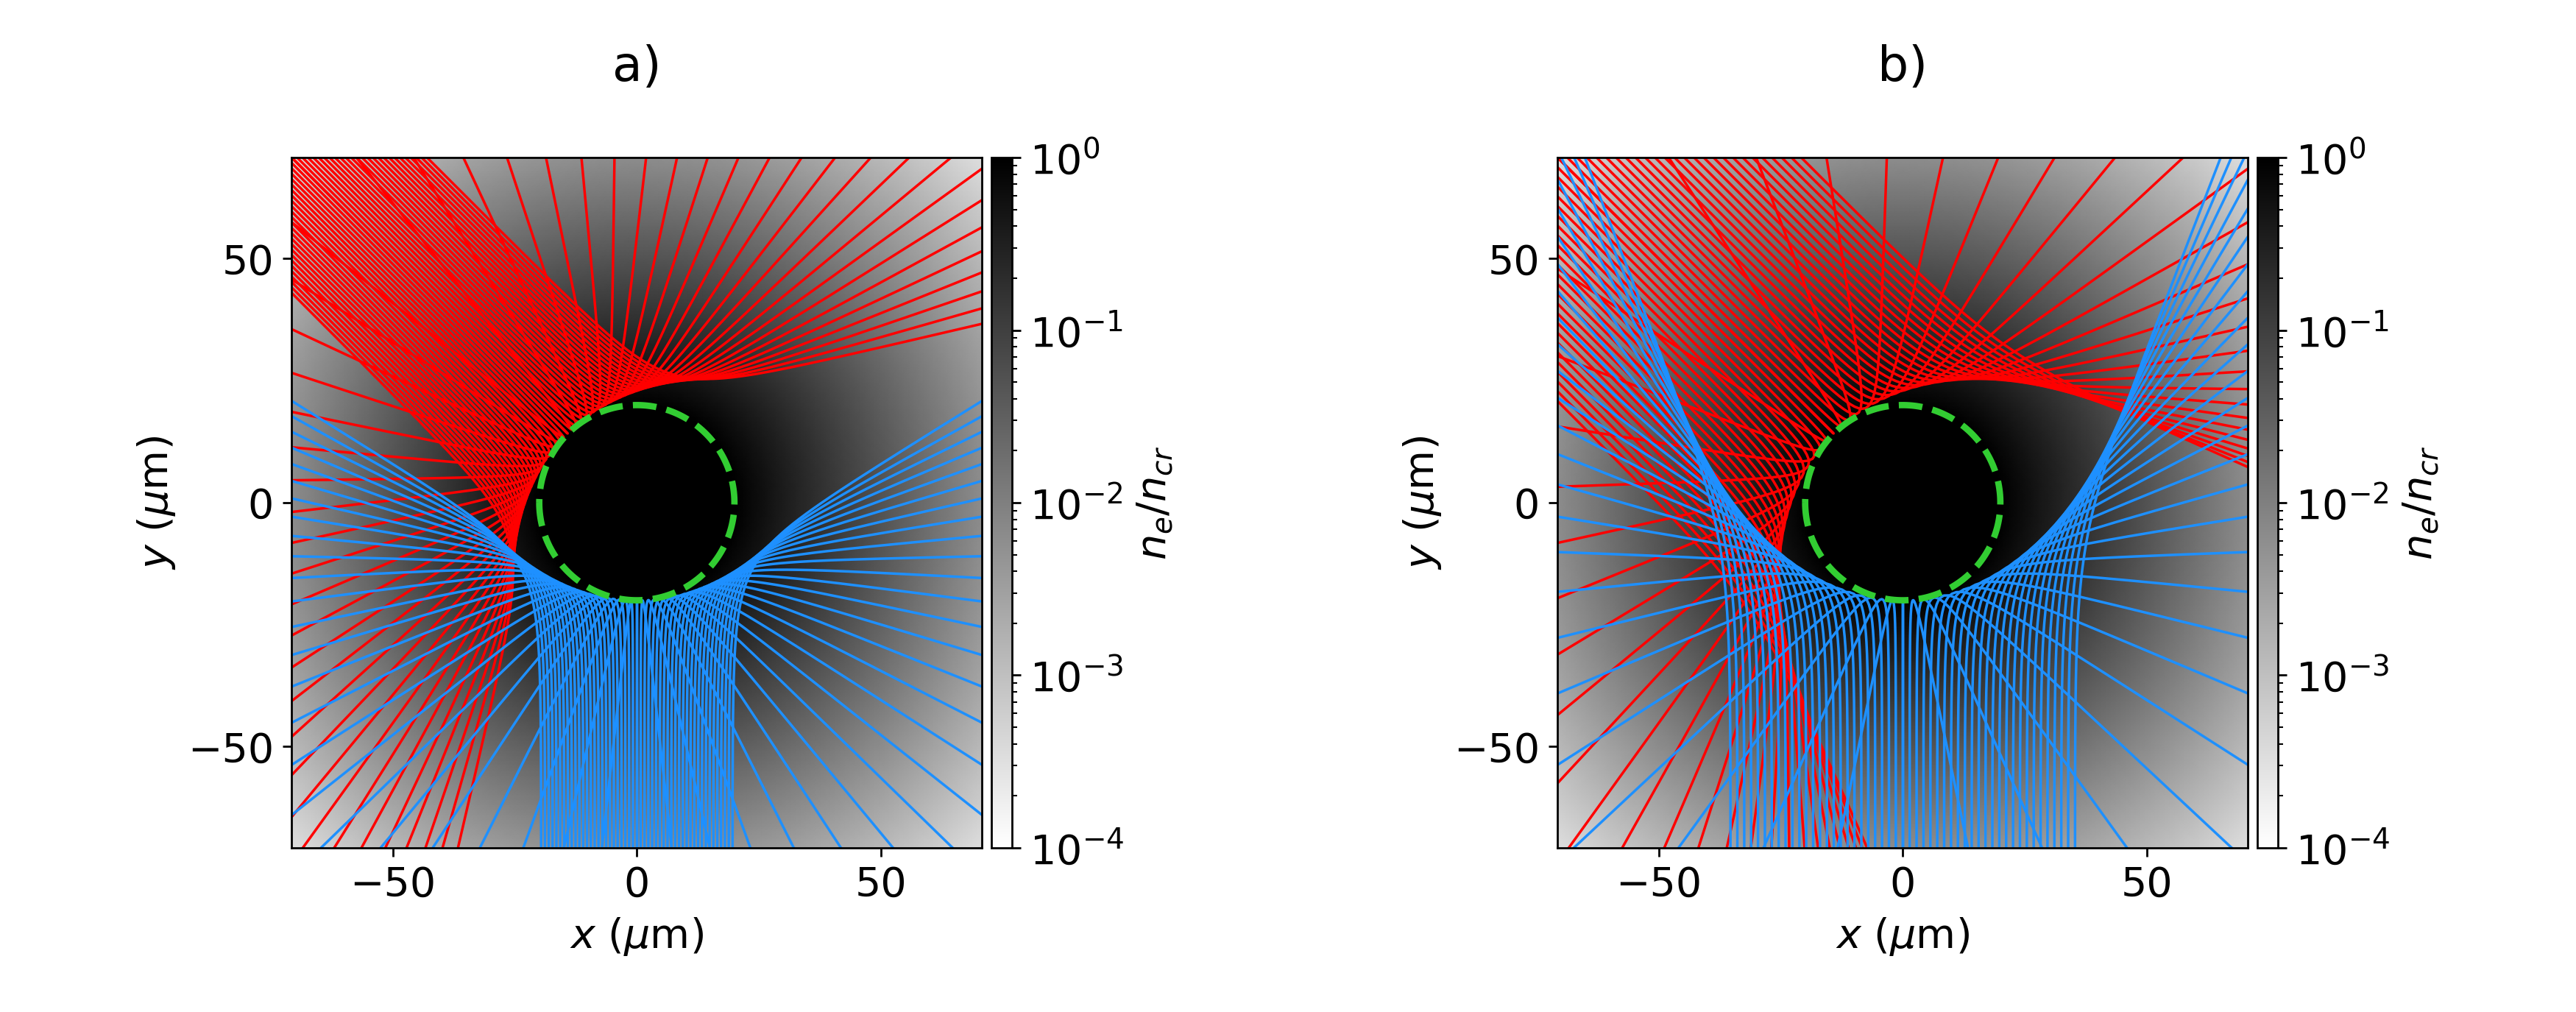
\includegraphics[width=\linewidth]{Results1/Images/RbRt_beam_overlap.png}
    \centering
    \caption{The trajectory of rays from two beams with Beam radii.
    The density profile for both simulations is $n_e=n_{\text{cr}}\exp{[ -(r_{\mu\text{m}}-20)/100 ]}$.
    Panels a) and b) plot rays from beams with widths $\sigma=10$ and $18\ \mu\text{m}$ respectively.}%
    \label{fig:Res1_RbRt_beam_overlap}
\end{figure}




%################################################################################
%################################################################################
\subsection{Statistical Modelling of \textsc{Omega} Direct-Drive Implosions}%
\label{sec:Res1_OMEGA_stat_modelling}


%################################################################################
%################################################################################
\subsection{Beam Radius in Statistical Modelling}%
\label{sec:Res1_OMEGA_stat_modelling_RbRt}


%###############################################################################################################################
%###############################################################################################################################
%###############################################################################################################################
\section{Cylindrical Simulation Platform for Beam Radius Parameter Scan}%
\label{sec:Res1_CylRbRt_platform}


%################################################################################
%################################################################################
\subsection{Assumptions and Validity of the Cylindrical Simulation Platform}%
\label{sec:Res1_platformvalidity}


%################################################################################
%################################################################################
\subsection{Problems with Traditional Methods of Investigating Beam Radius Parameter Computationally}%
\label{sec:Res1_computational_difficulties}


%################################################################################
%################################################################################
\subsection{Pulse Shape and Target Initial Conditions}%
\label{sec:Res1_initialconditions}

\begin{figure}[t!]
    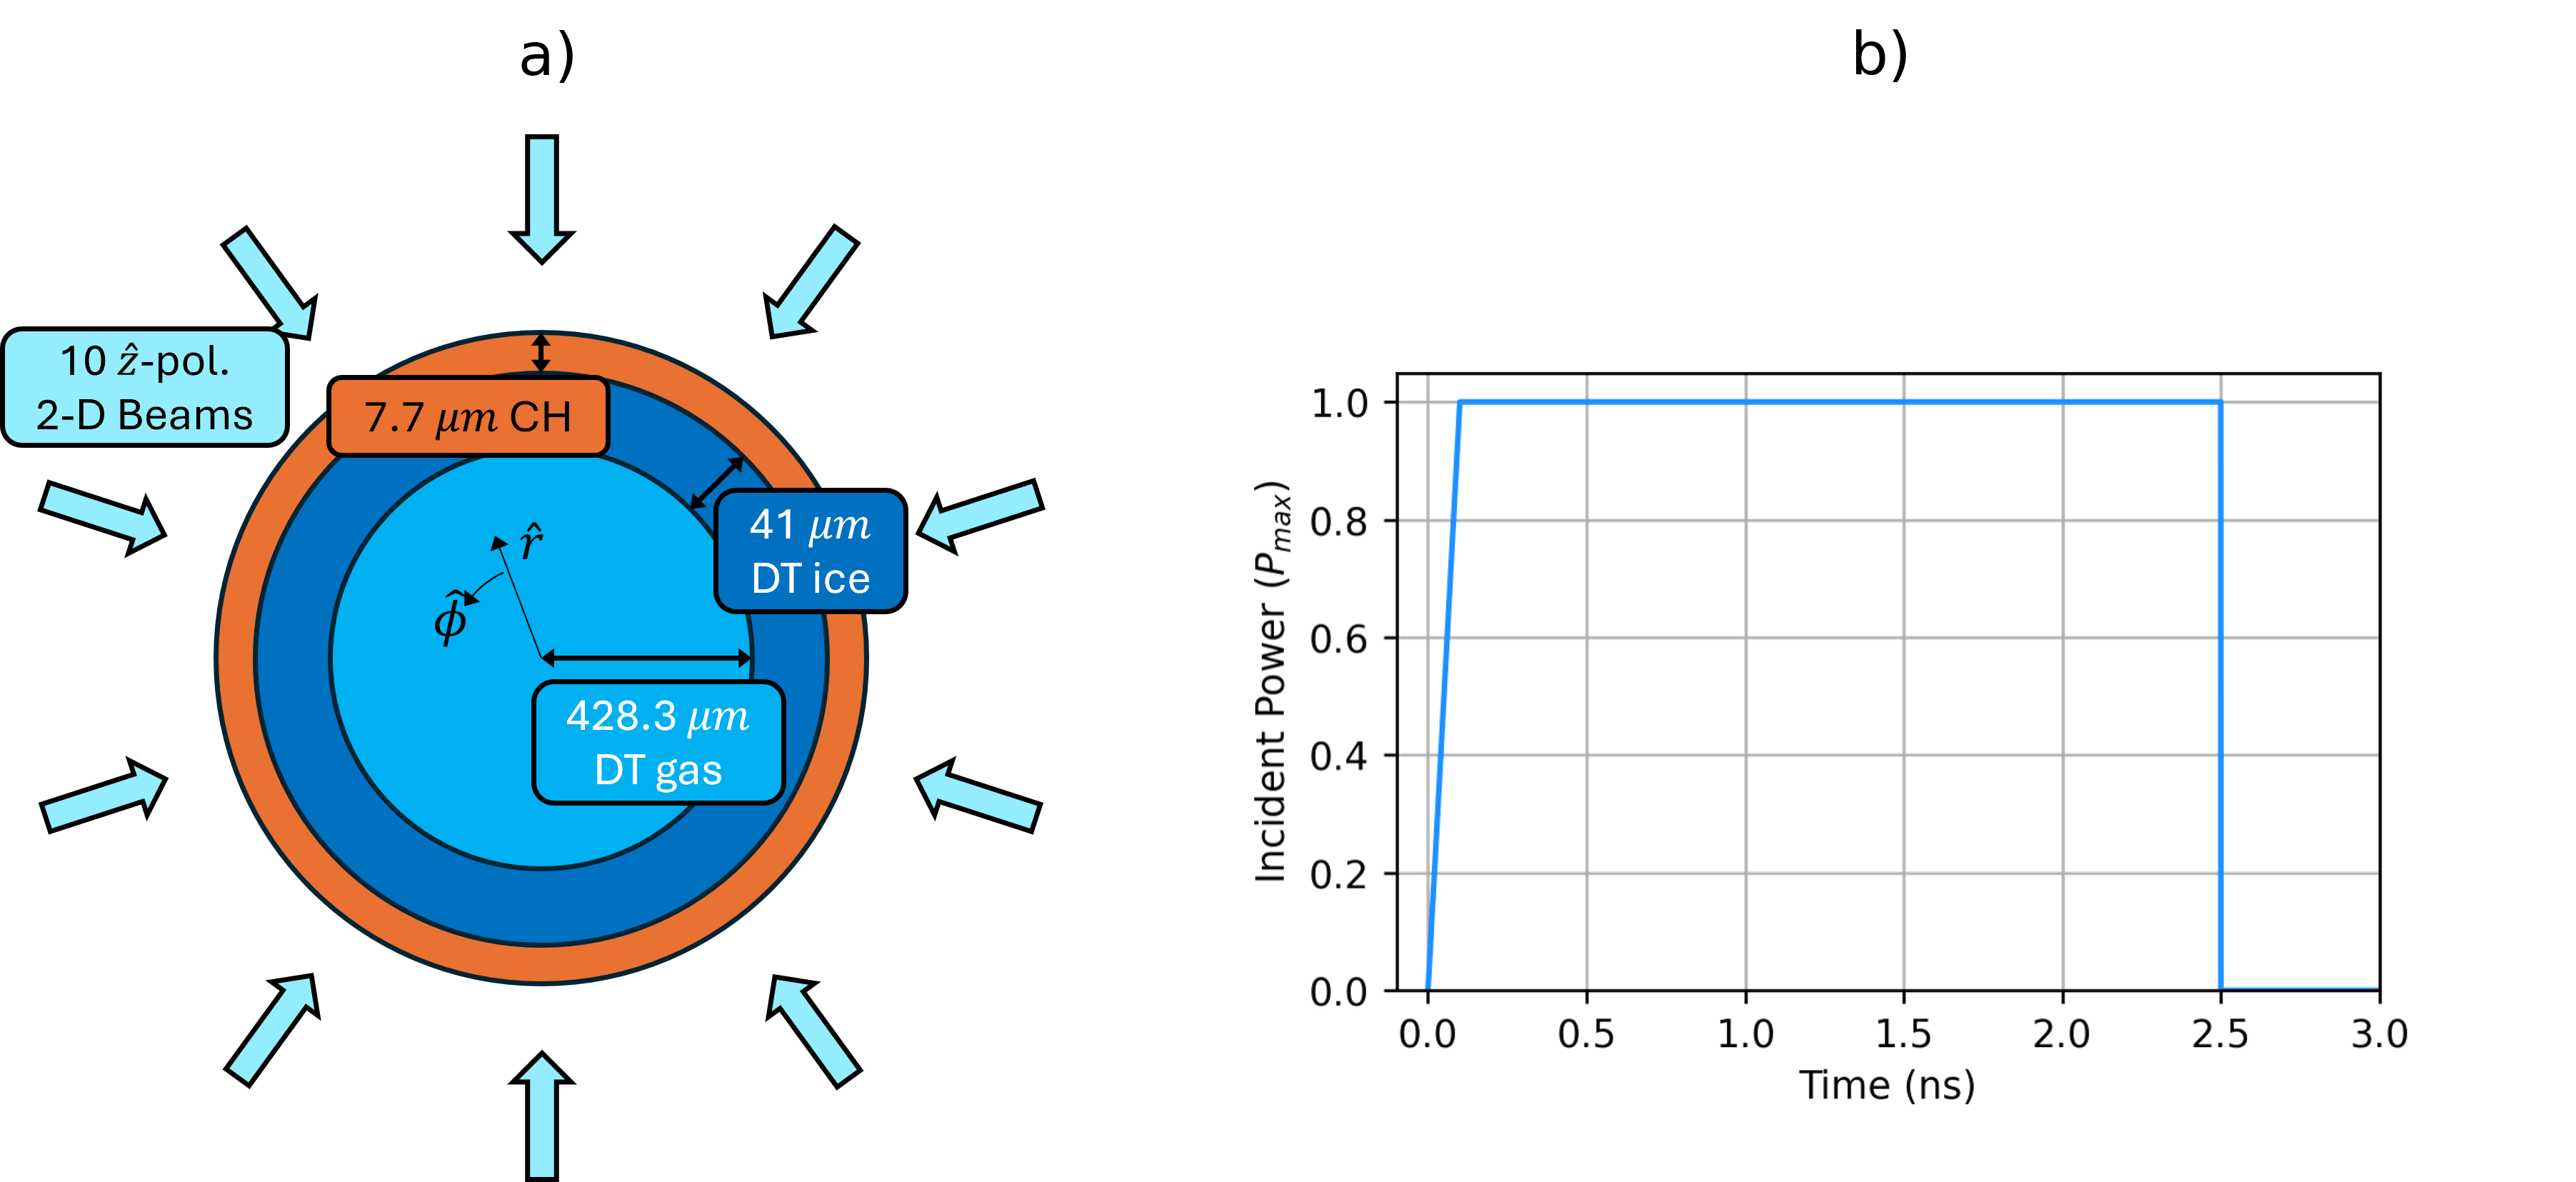
\includegraphics[width=\linewidth]{Results1/Images/cyl_setup.png}
    \centering
    \caption{The target initial conditions with beam geometry, a), and pulse shape, b), used for the 2-D cylindrical simulations.
    All beams were polarised out of the simulation plane, in the $+\hat{\vec{z}}$ direction.
    Initial layer radii were taken from the initial conditions for \textsc{Omega} shot 89224, presented in Fig.~\ref{fig:89224_ICs}.a.}%
    \label{fig:Res1_cyl_setup}
\end{figure}


%################################################################################
%################################################################################
\subsection{1-D Implosion Tuning}%
\label{sec:Res1_1D_tuning}

\bgroup
\def\arraystretch{1.2}%  1 is the default, change whatever you need
% Please add the following required packages to your document preamble:
% \usepackage{multirow}
\begin{table}[]
    \centering
    \caption{Results of the 1-D Tuning Simulations.}
    \begin{tabular}{cccccc}
    \hhline{======}
    $R_b/R_t$             &         & \begin{tabular}[c]{@{}c@{}}$P_{\text{max}}$\\ ($\text{TW}/\text{cm}$)\end{tabular} & \begin{tabular}[c]{@{}c@{}}$I_0$\\ ($10^{14}\ \text{W}/\text{cm}^2$)\end{tabular} & \begin{tabular}[c]{@{}c@{}}$t_{\text{bang}}$\\ ($\text{ns}$)\end{tabular} & \begin{tabular}[c]{@{}c@{}}$Y_{\text{DT}}$\\ ($10^{13}\ /\text{cm}$)\end{tabular} \\ \hhline{======}
    \multirow{2}{*}{0.75} & No CBET & \multirow{2}{*}{54.44}                                                             & \multirow{2}{*}{0.85}                                                   & 2.49                                                                      & 1.53                                 \\
                          & CBET    &                                                                                    &                                                                         & 2.51                                                                      & 1.44                                 \\ \hline
    \multirow{2}{*}{0.80} & No CBET & \multirow{2}{*}{58.25}                                                             & \multirow{2}{*}{0.83}                                                   & 2.49                                                                      & 1.56                                 \\
                          & CBET    &                                                                                    &                                                                         & 2.51                                                                      & 1.45                                 \\ \hline
    \multirow{2}{*}{0.85} & No CBET & \multirow{2}{*}{63.44}                                                             & \multirow{2}{*}{0.83}                                                   & 2.48                                                                      & 1.67                                 \\
                          & CBET    &                                                                                    &                                                                         & 2.51                                                                      & 1.43                                 \\ \hline
    \multirow{2}{*}{0.90} & No CBET & \multirow{2}{*}{70.00}                                                             & \multirow{2}{*}{0.85}                                                   & 2.47                                                                      & 1.82                                 \\
                          & CBET    &                                                                                    &                                                                         & 2.50                                                                      & 1.41                                 \\ \hline
    \multirow{2}{*}{0.95} & No CBET & \multirow{2}{*}{77.94}                                                             & \multirow{2}{*}{0.89}                                                   & 2.46                                                                      & 1.99                                 \\
                          & CBET    &                                                                                    &                                                                         & 2.49                                                                      & 1.49                                 \\ \hline
    \multirow{2}{*}{1.00} & No CBET & \multirow{2}{*}{87.25}                                                             & \multirow{2}{*}{0.93}                                                   & 2.45                                                                      & 2.15                                 \\
                          & CBET    &                                                                                    &                                                                         & 2.49                                                                      & 1.60                                 \\ \hline
    \multirow{2}{*}{1.05} & No CBET & \multirow{2}{*}{97.94}                                                             & \multirow{2}{*}{0.99}                                                   & 2.46                                                                      & 2.27                                 \\
                          & CBET    &                                                                                    &                                                                         & 2.50                                                                      & 1.61                                 \\ \hline
    \multirow{2}{*}{1.10} & No CBET & \multirow{2}{*}{110.00}                                                            & \multirow{2}{*}{1.06}                                                   & 2.47                                                                      & 2.31                                 \\
                          & CBET    &                                                                                    &                                                                         & 2.51                                                                      & 1.52                                 \\ \hhline{======}
    \end{tabular}
    \label{tab:res1_1d_tuning}
\end{table}
\egroup

\begin{figure}[t!]
    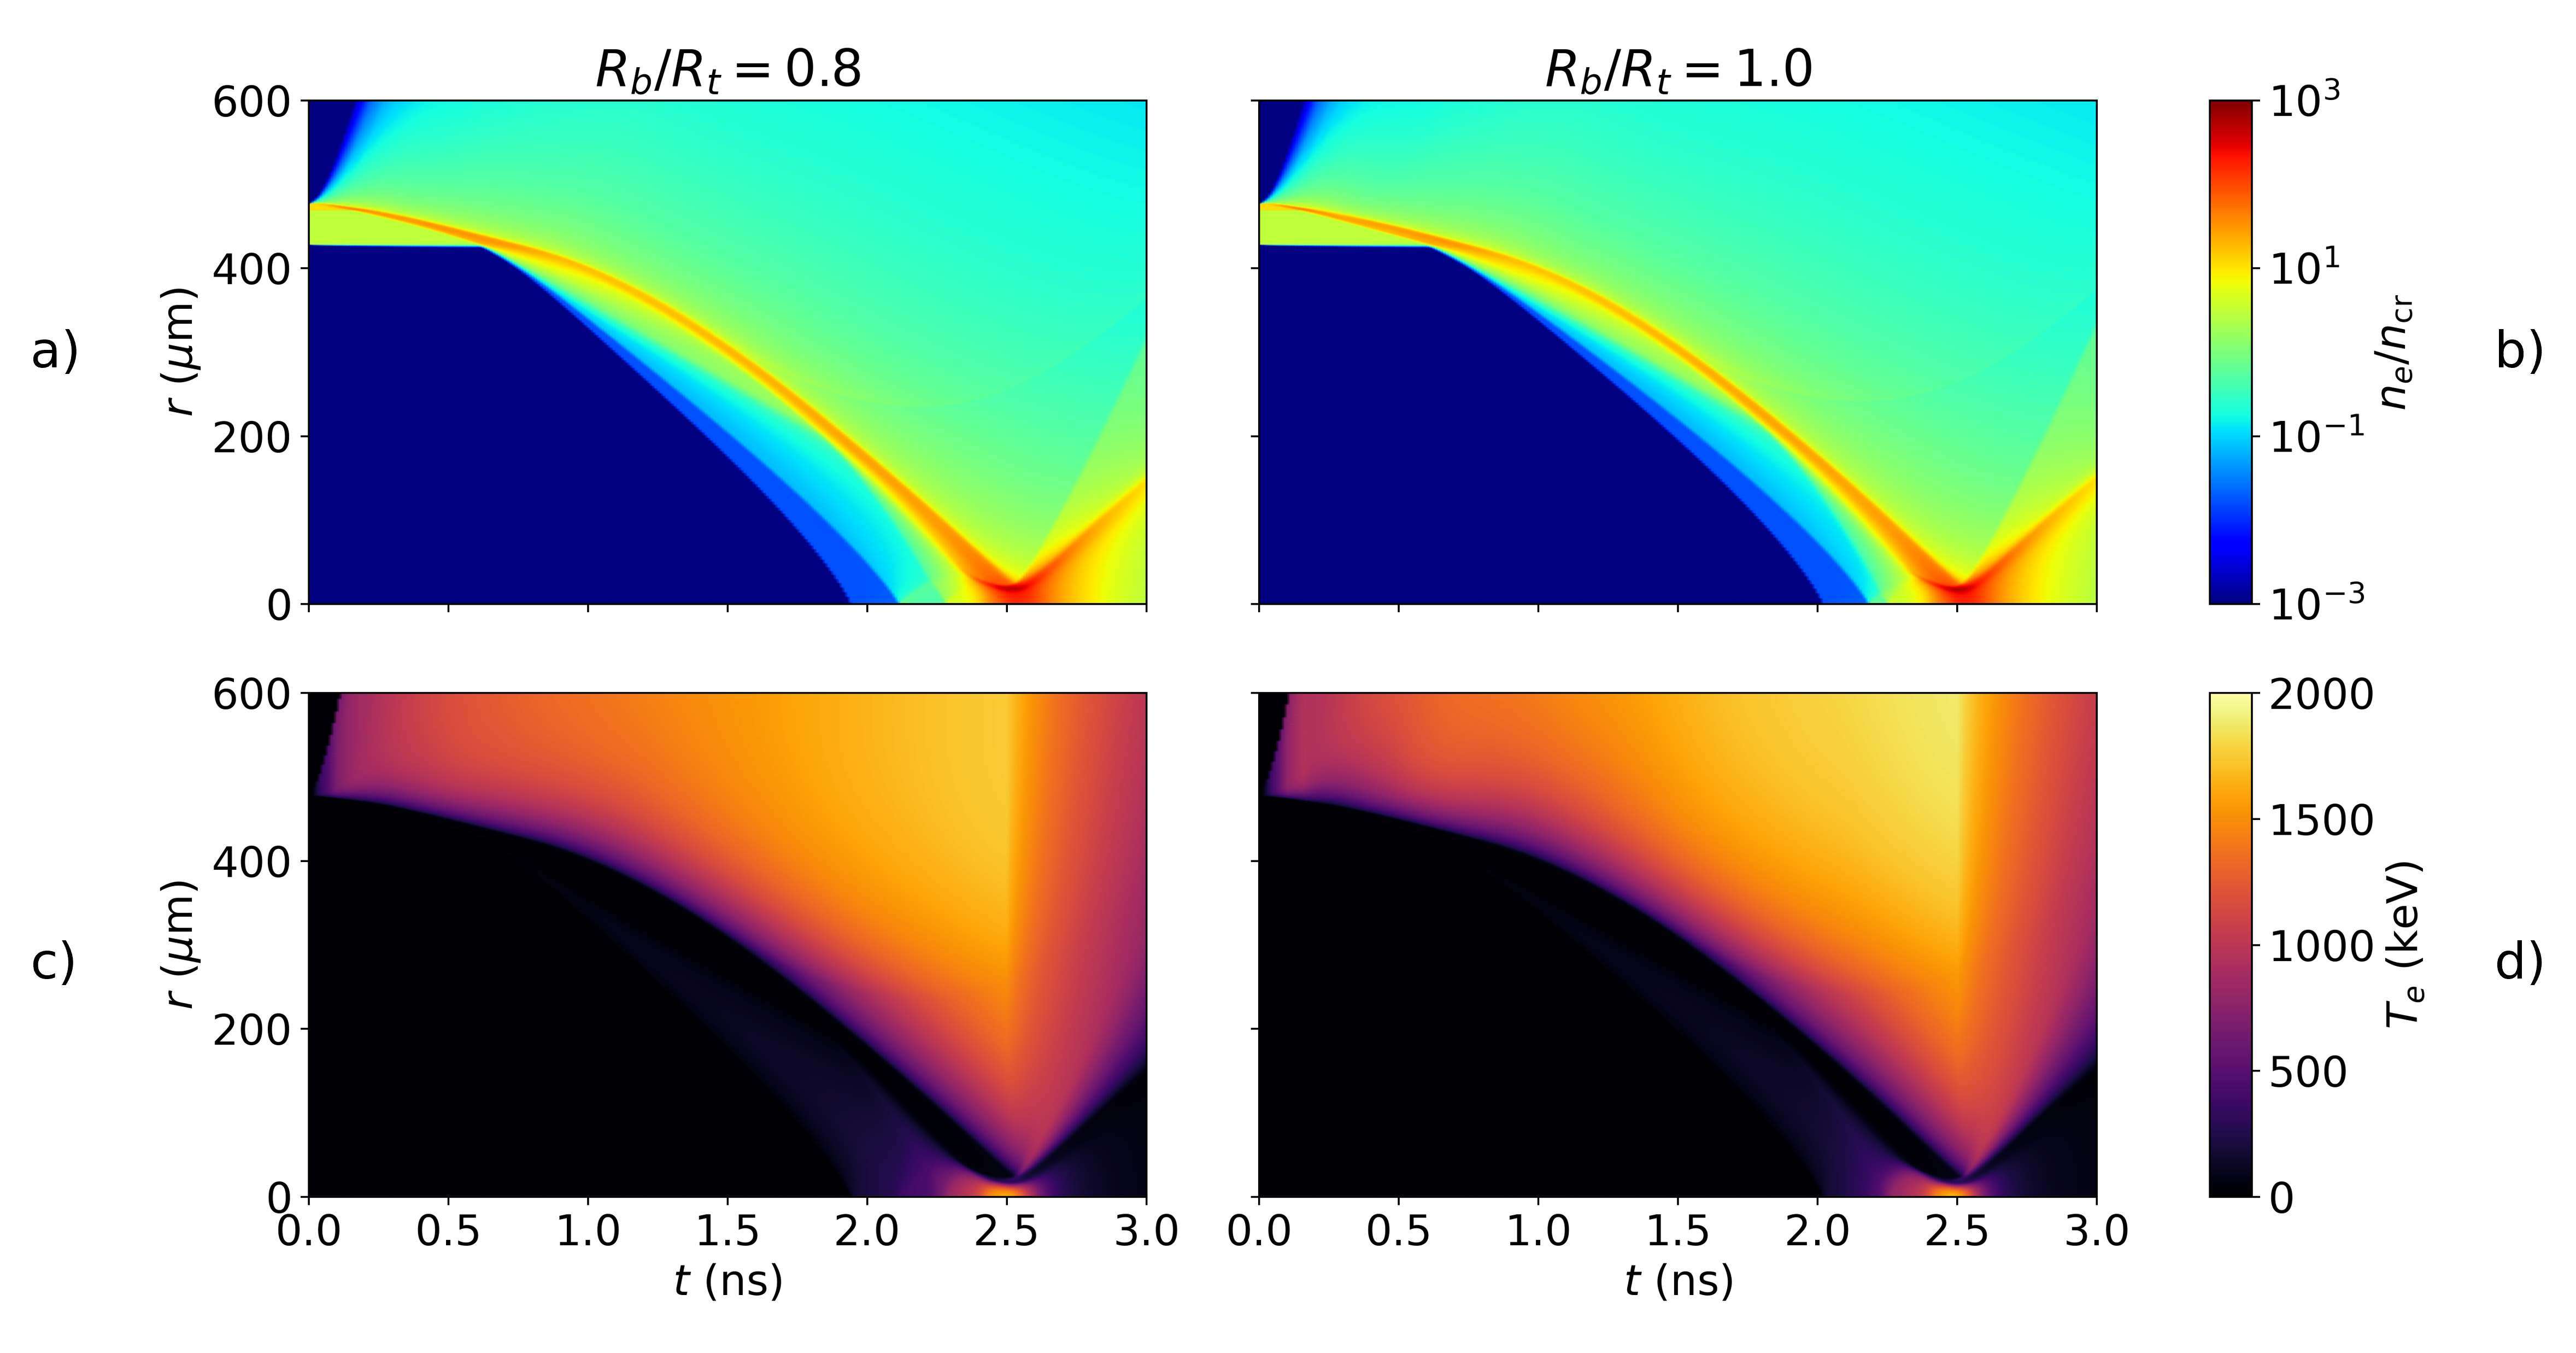
\includegraphics[width=\linewidth]{Results1/Images/streaks.png}
    \centering
    \caption{Streak plots from two of the 1-D tuning simulations.
    Panels a) \& b) plot the electron density as a function of time ($x$-axis) and radius ($y$-axis) for the \ac{CBET} simulations of the $R_b/R_t=0.8$ \& $R_b/R_t=1.0$ simulations respectively.
    Panels c) \& d) plot the same but electron temperature for the $R_b/R_t=0.8$ \& $R_b/R_t=1.0$ simulations respectively.}%
    \label{fig:Res1_streaks}
\end{figure}


%###############################################################################################################################
%###############################################################################################################################
%###############################################################################################################################
\section{CBET Induced Modal Flips in Power Deposition Asymmetries}%
\label{sec:Res1_PdepR_CBET_asymm}


%################################################################################
%################################################################################
\subsection{Deposition Asymmetries in the Absence of CBET}%
\label{sec:Res1_noCBET_asymmetries}

\begin{figure}[t!]
    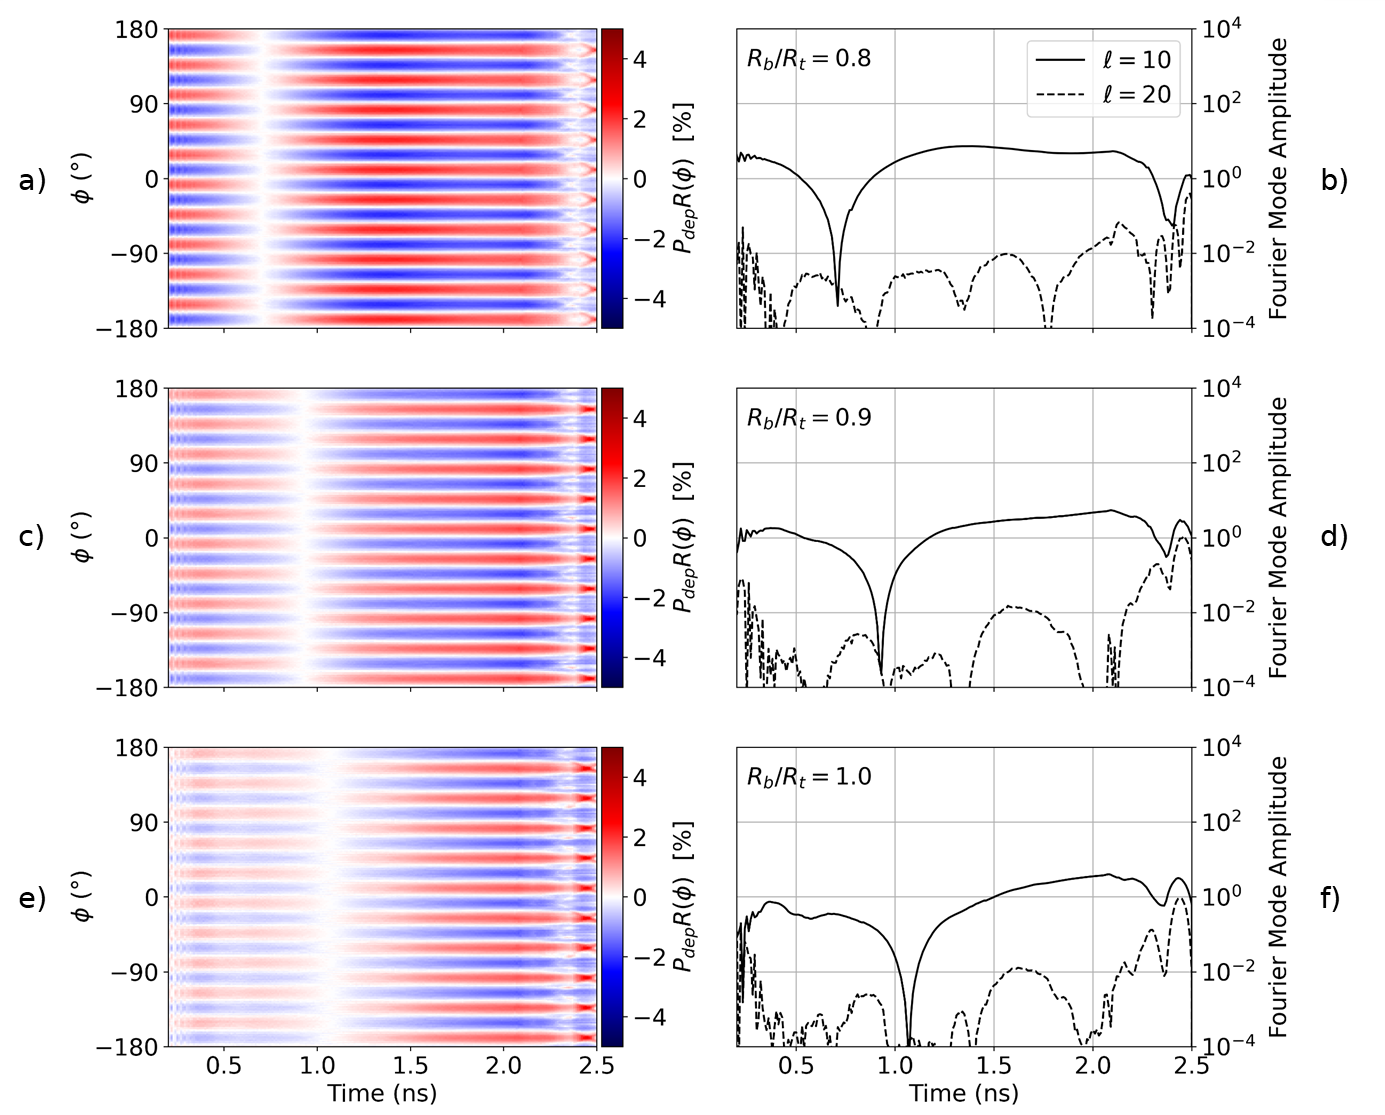
\includegraphics[width=\linewidth]{Results1/Images/noCBET_PR_modes.png}
    \centering
    \caption{This figure plots the radially integrated deposited power from no \ac{CBET} simulations as a function of time ($x$-axis) and angle ($y$-axis), alongside amplitudes of the dominant modes from a Fourier power spectrum.
    Panels a) and b) plot the radially integrated deposited power and Fourier modes respectively for the $R_b/R_t=0.8$ simulation.
    The same is plotted for the $R_b/R_t=0.9$ simulation in c) \& d) and for the $R_b/R_t=1.0$ simulation in e) \& f).
    The mode 10 from the number of beams is clearly visible in the radially integrated power plots as 10 peaks to troughs in angle at a given time, \textit{i.e.} 10 cyclical perturbations along a vertical lineout.}%
    \label{fig:Res1_PR_noCBET_modes}
\end{figure}


%################################################################################
%################################################################################
\subsection{CBET Imprint on Incident Field}%
\label{sec:Res1_CBET_imprint}

\begin{figure}[t!]
    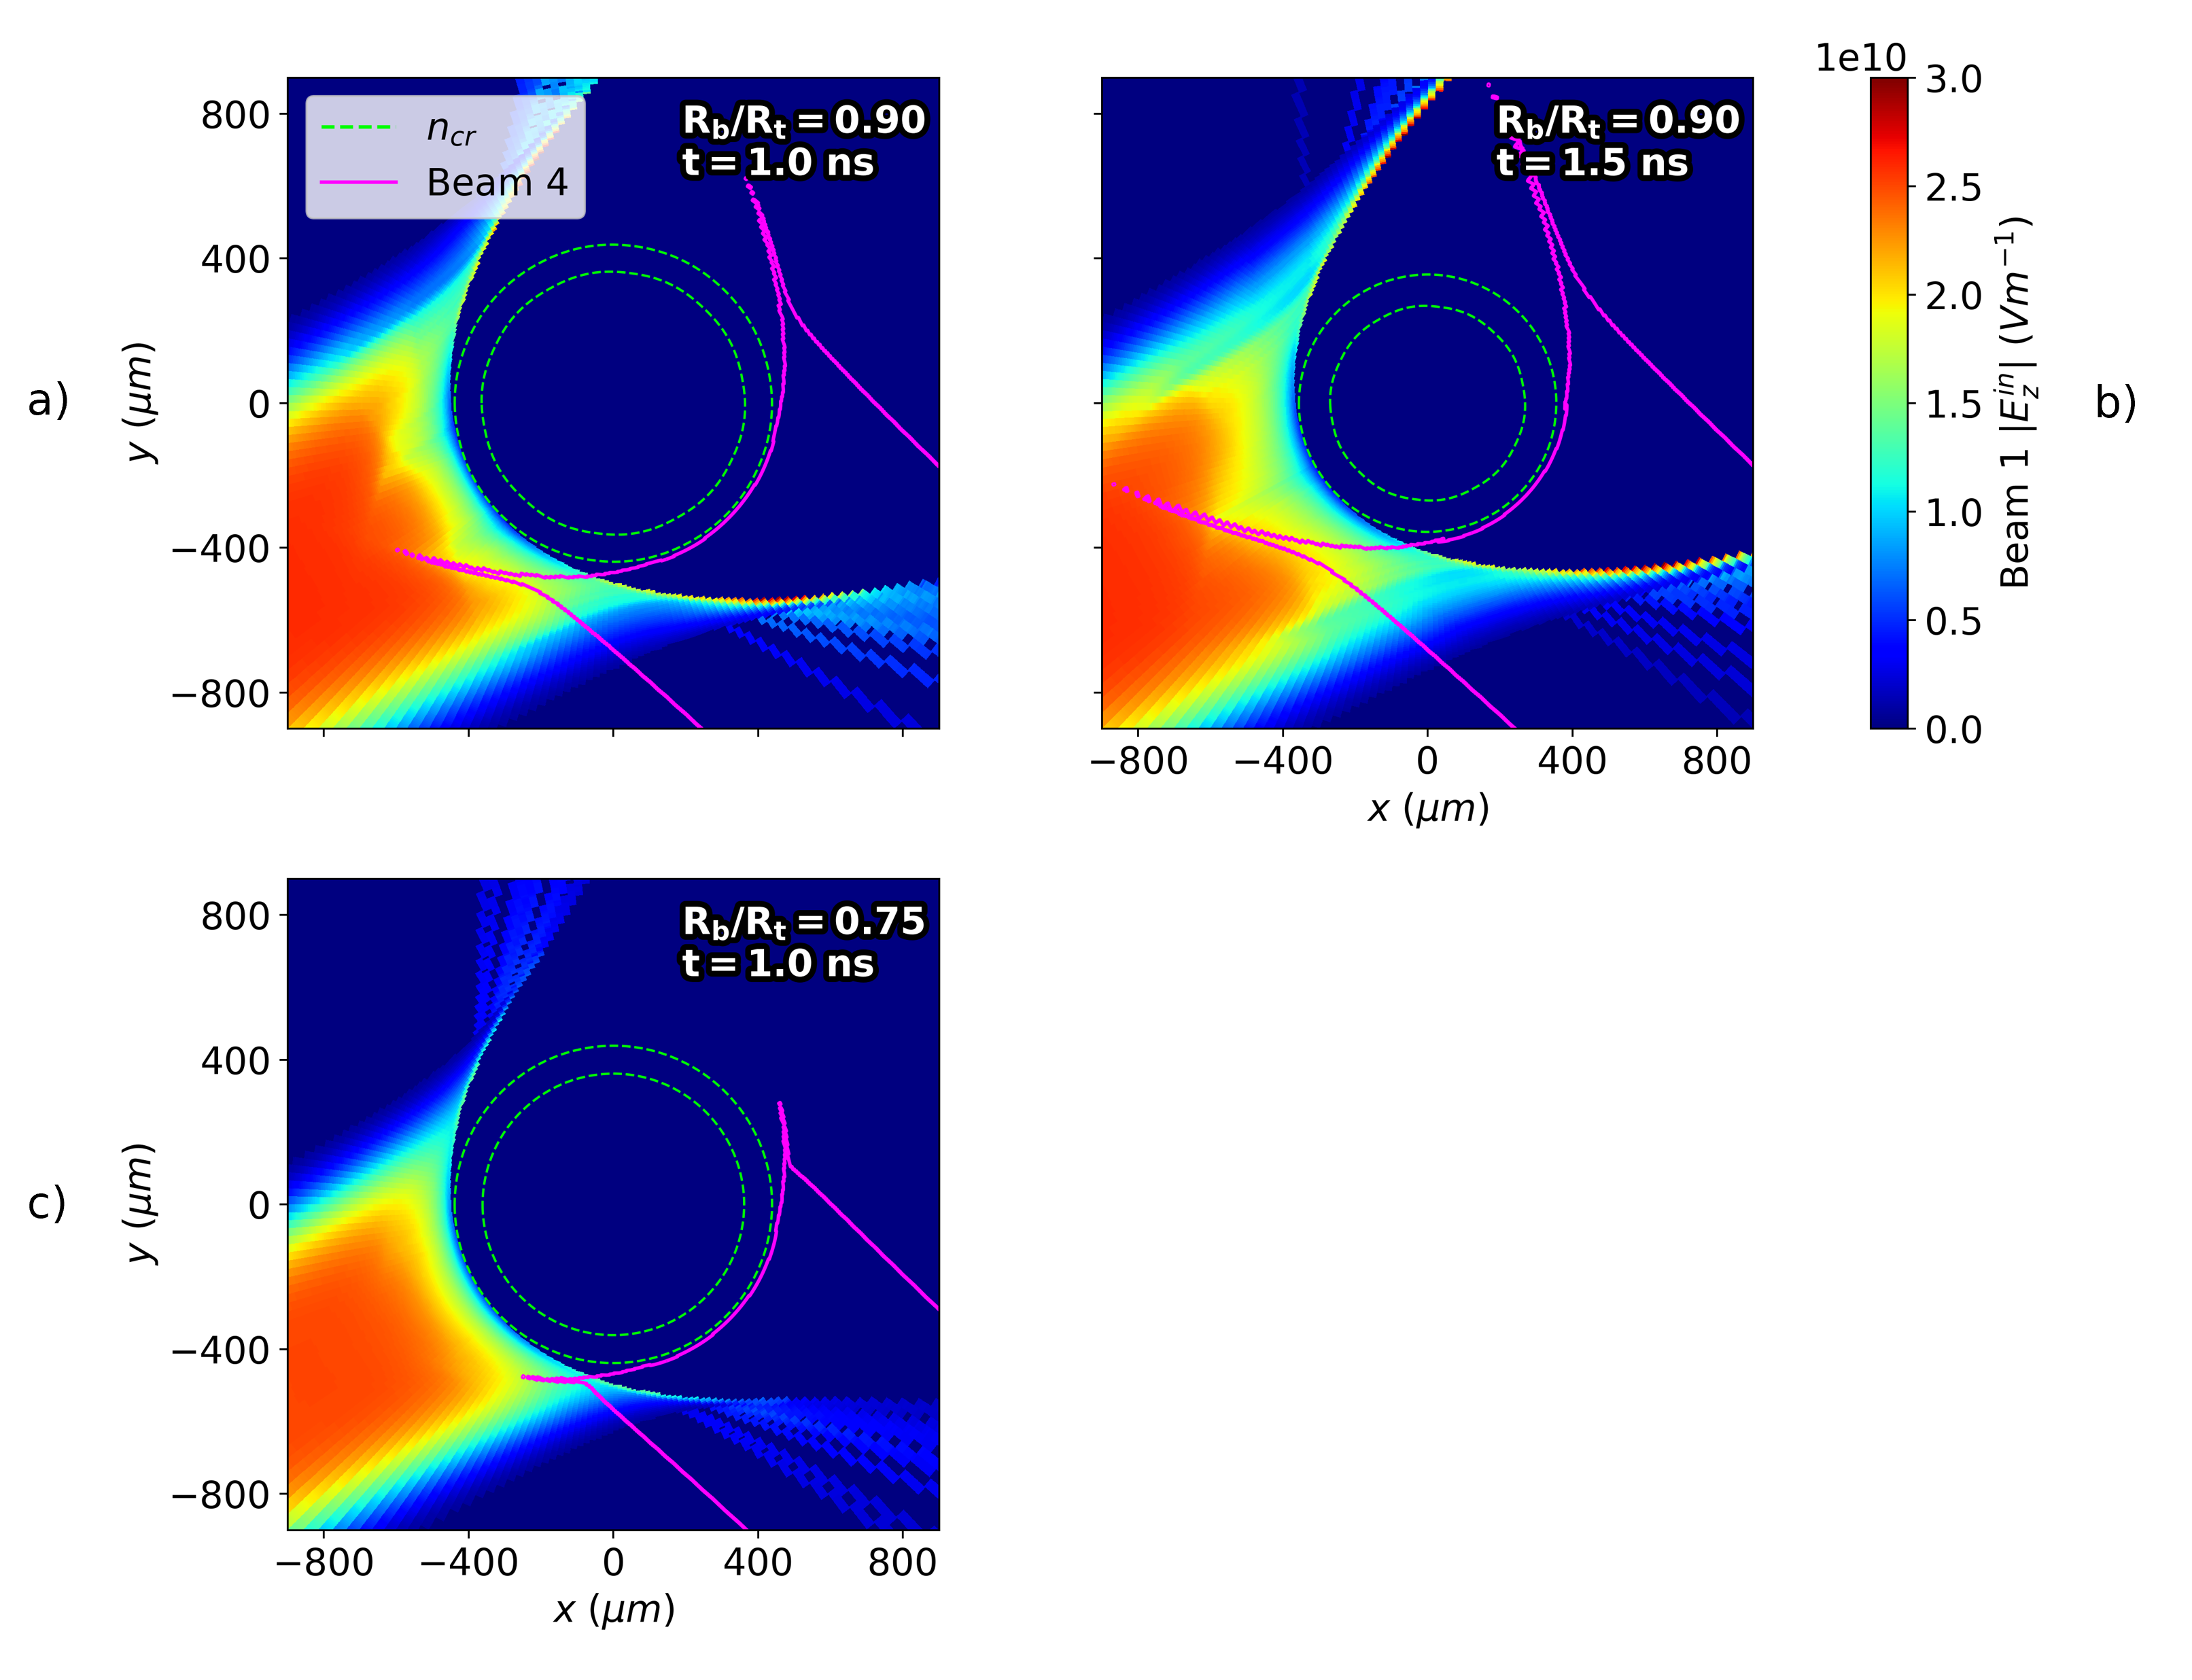
\includegraphics[width=\linewidth]{Results1/Images/Field_profiles.png}
    \centering
    \caption{This plot illustrates the origin of the \ac{CBET} induced asymmetry on power deposition and its dependence on $R_b/R_t$ and target convergence.
    Each panel plots the incident field (including the effect of \ac{CBET}), along with contours of the critical electron density and the $|E_z^{\text{in}}|=1\times10^{10}\ \text{Vm}^{-1}$ contour of another beam.
    Panel a) \& b) plot this for the $R_b/R_t=0.9$ simulation at $t=1.0\ \text{ns}$ \& $t=1.5\ \text{ns}$ respectively.
    The convergence of the target in this time interval leads to greater convergence and therefore a change in the spatial location across the beam of the resonant \ac{CBET} interaction.
    Panel c) plots the $R_b/R_t=0.75$ at the same time as panel a).
    This demonstrates that the $R_b/R_t=0.75$ beam is not wide enough at this time to lead to a resonant \ac{CBET} interaction, unlike the wider beam in panel a).}%
    \label{fig:Res1_field_profiles}
\end{figure}


%################################################################################
%################################################################################
\subsection{Modal Flips of Power Deposition Asymmetries}%
\label{sec:Res1_ModalFlip}

\begin{figure}[t!]
    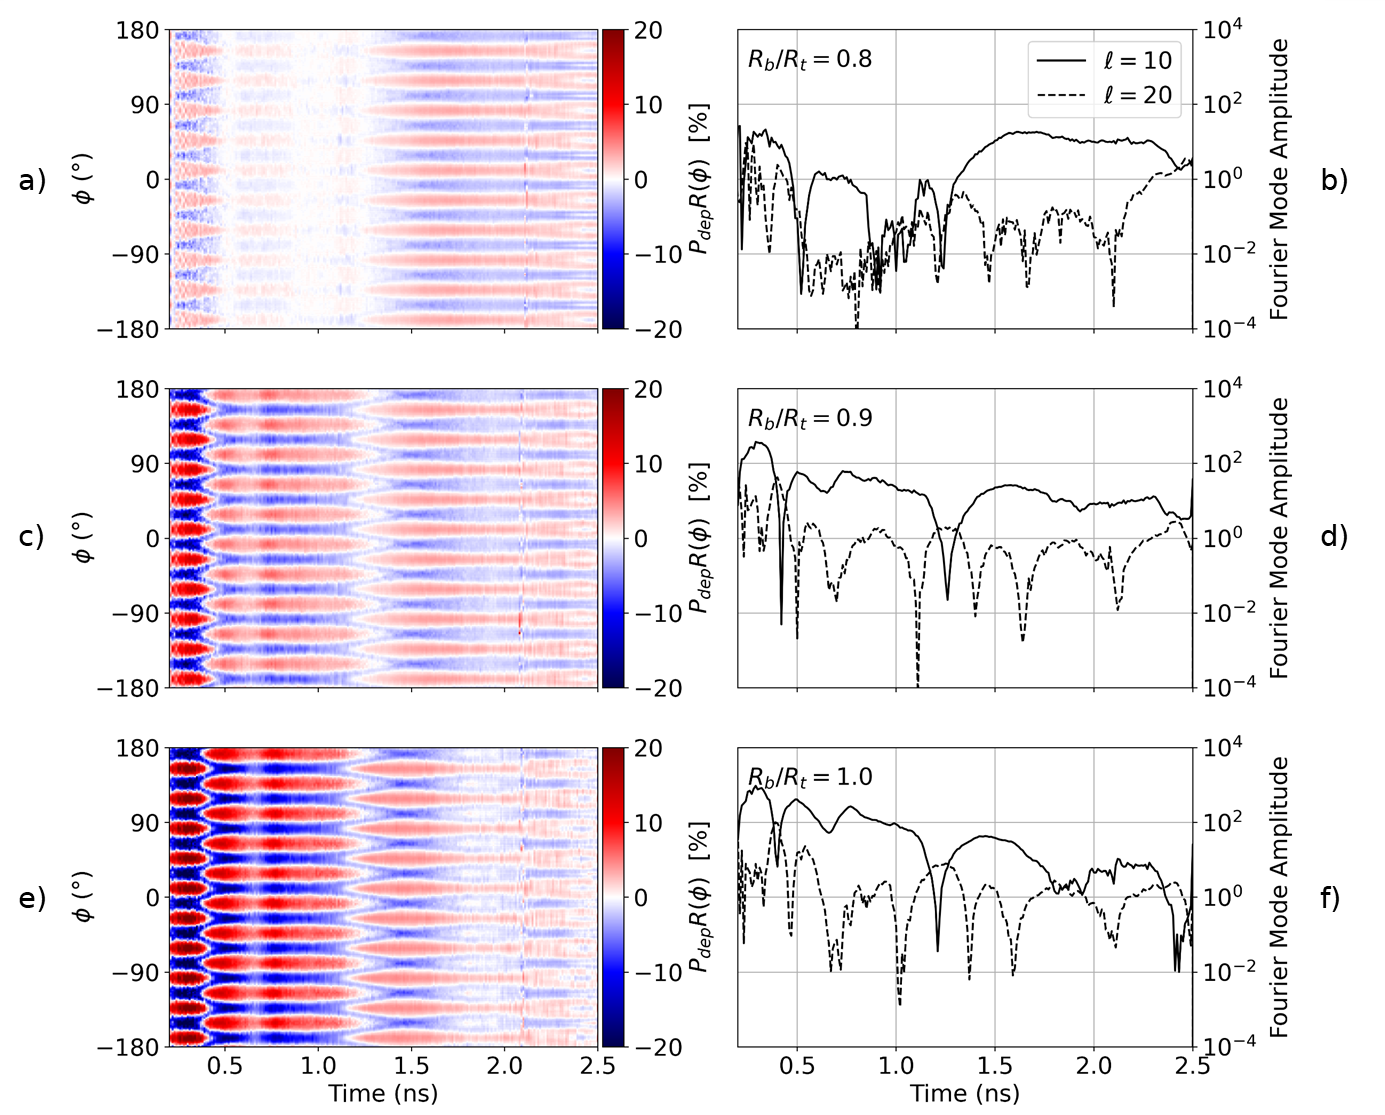
\includegraphics[width=\linewidth]{Results1/Images/CBET_PR_modes.png}
    \centering
    \caption{This figure plots the same as Fig.~\ref{fig:Res1_PR_noCBET_modes}, but now for the equivalent simulation including the effect of \ac{CBET}.
    Comparing these results and those in Fig.~\ref{fig:Res1_PR_noCBET_modes} demonstrates that \ac{CBET} introduces additional modal-flips of the deposition and amplifies the magnitude of asymmetries.}%
    \label{fig:Res1_PR_CBET_modes}
\end{figure}


%###############################################################################################################################
%###############################################################################################################################
%###############################################################################################################################
\section{Stagnation State Asymmetry}%
\label{sec:Res1_StagnationAsymm}


%################################################################################
%################################################################################
\subsection{Hotspot Profiles}%
\label{sec:Res1_HS_profiles}

\begin{figure}[t!]
    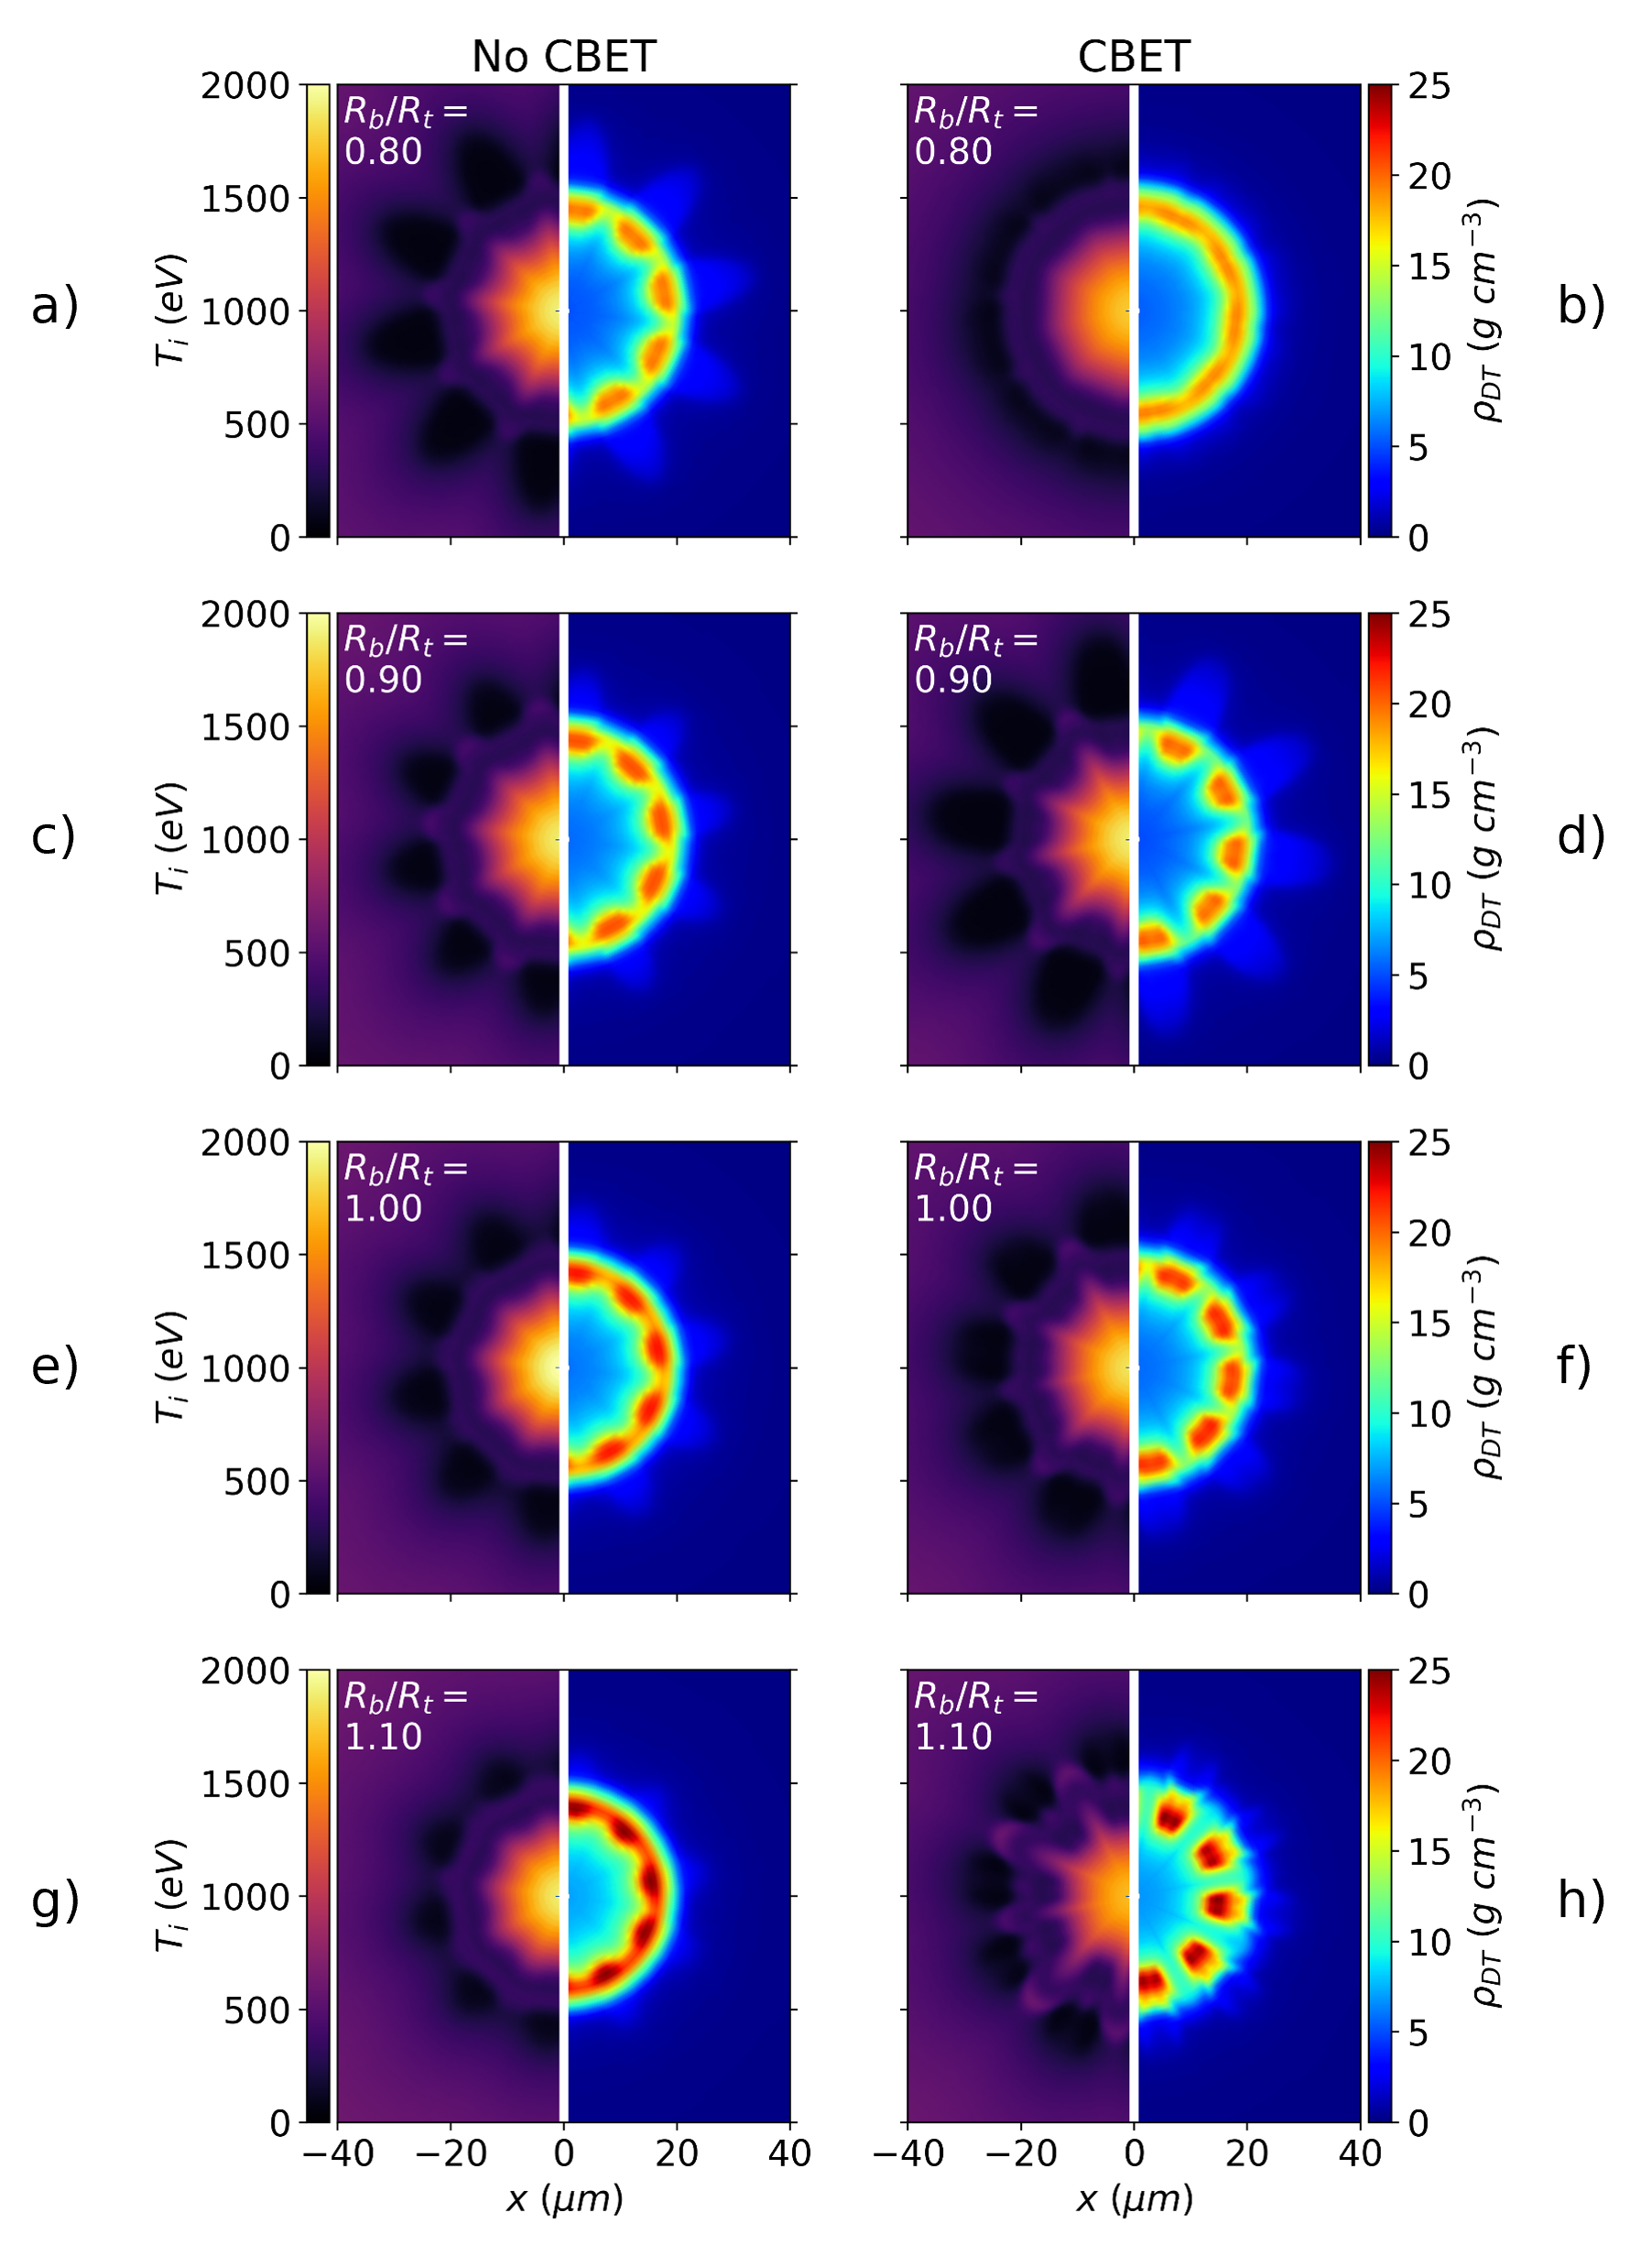
\includegraphics[width=0.8\linewidth]{Results1/Images/Stagnation_plots.png}
    \centering
    \caption{Densities of the DT fuel and ion temperatures for various $R_b/R_t$ simulations both with and without \ac{CBET}.
    Each row correspond to a different $R_b/R_t$ value; the left column contains simulations without \ac{CBET}; and the right column contains simulations with \ac{CBET}.
    It is visible from the density plots that increasing $R_b/R_t$ improves stagnation symmetry for the no \ac{CBET} simulations, but degrades it for the \ac{CBET} simulations.}%
    \label{fig:Res1_stagnation_plots}
\end{figure}



%################################################################################
%################################################################################
\subsection{Stagnation State Asymmetry Trend with Beam Radius}%
\label{sec:Res1_stagnation_asymm_trend}

\begin{figure}[t!]
    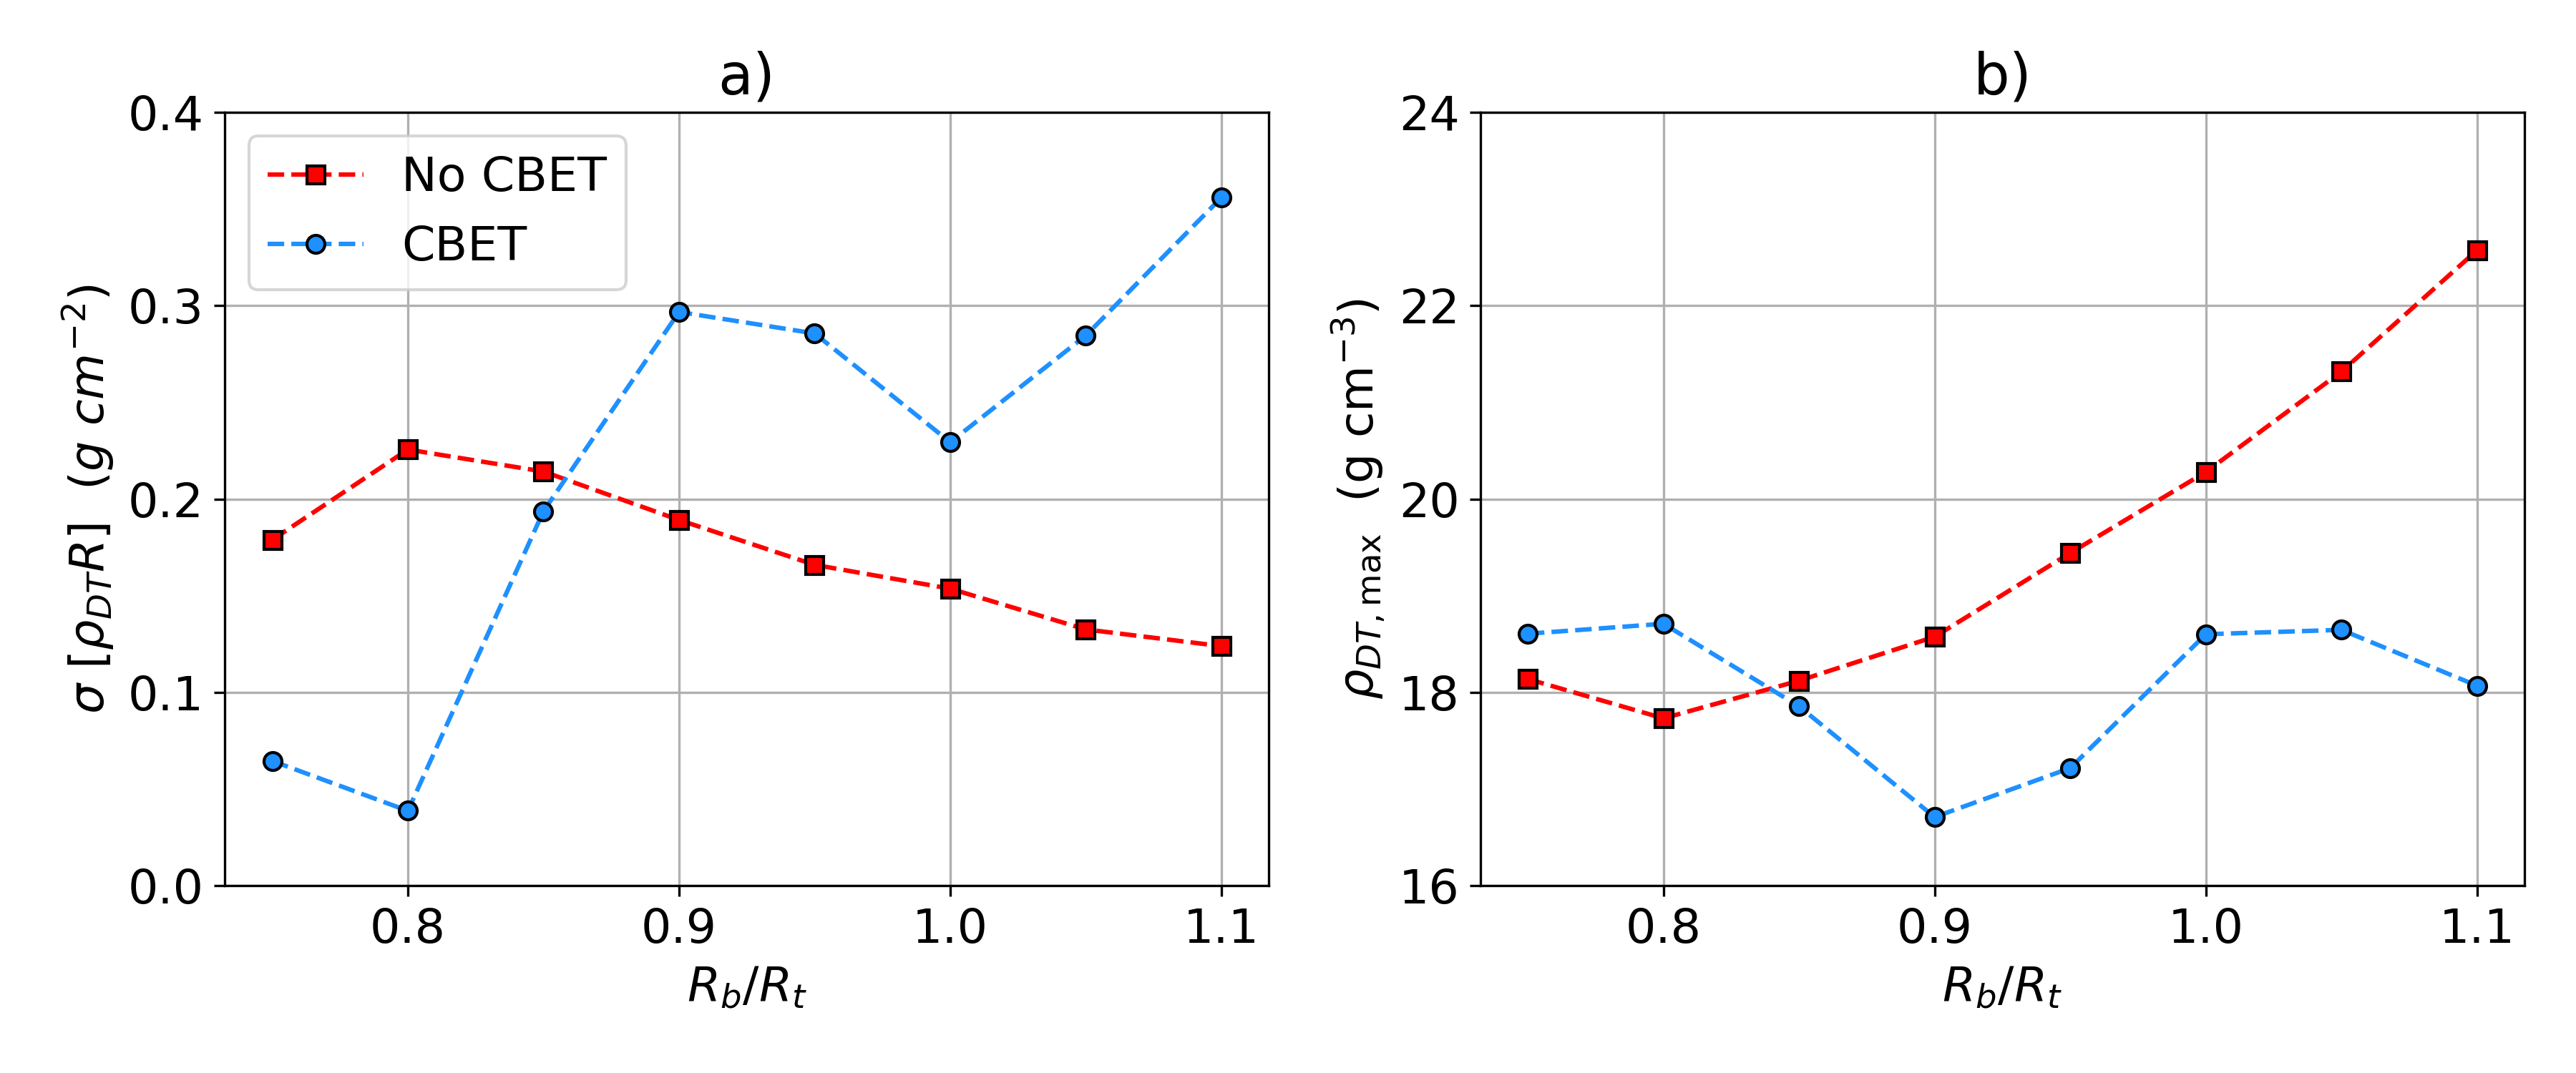
\includegraphics[width=1.0\linewidth]{Results1/Images/RbRt_sig_rhomax.png}
    \centering
    \caption{Trends of a) stagnation asymmetry and b) maximum (azimuthally averaged) fuel density for \ac{CBET} and no \ac{CBET} simulations.
    The no \ac{CBET} improvement in symmetry with $R_b/R_t$ is observed which also corresponds to improved compression.
    The symmetry trend including \ac{CBET} is more complex, but broadly the stagnation state symmetry is worse with increasing $R_b/R_t$.}%
    \label{fig:Res1_asymm_trend}
\end{figure}


%################################################################################
%################################################################################
\subsection{Time Resolved Asymmetry Growth}%
\label{sec:Res1_time_res_growth}

\begin{figure}[t!]
    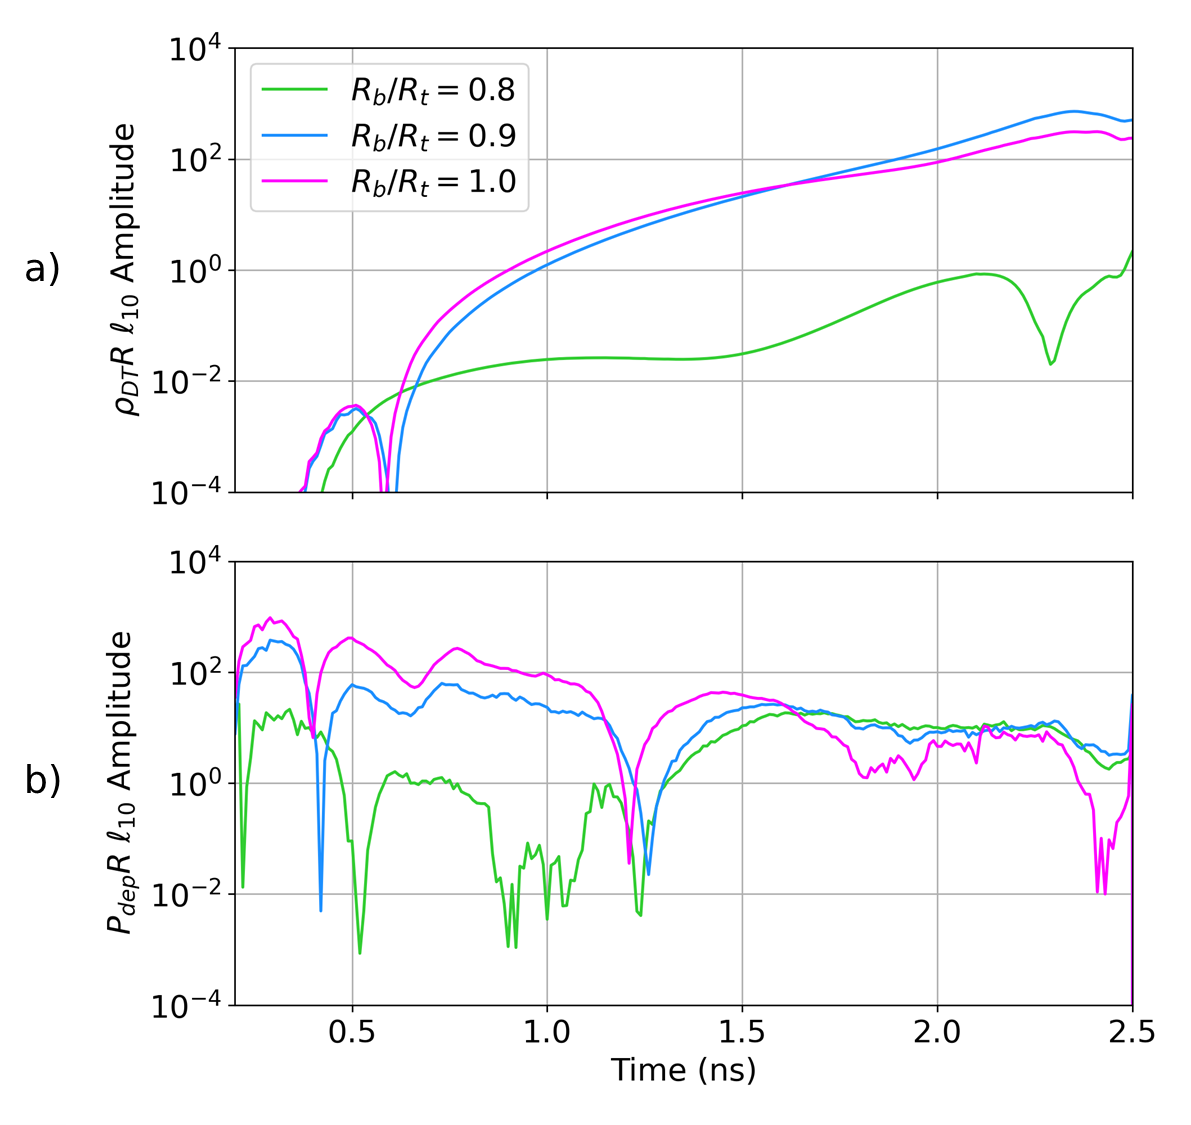
\includegraphics[width=0.75\linewidth]{Results1/Images/RbRts_mode10_growth.png}
    \centering
    \caption{Time resolved $\ell=10$ Fourier power spectrum amplitude for a) $\rho_{\text{DT}}R$ and b) $P_{\text{dep}}R$ for \ac{CBET} simulations with 3 $R_b/R_t$ values.
    The developing but unrealised modal flip for $R_b/R_t=0.8$ from $t \sim 0.5\rightarrow 1.2\ \text{ns}$ reduces the $P_{\text{dep}}R_{\ell=10}$ leading to slow $\rho_{\text{DT}}R_{\ell=10}$ growth and ultimately a relatively symmetric stagnation state.
    %Note that this developing but unrealised modal flip is clearly visible from reduced $P_{\text{dep}}R$ asymmetry values in Fig.~\ref{fig:Res1_PR_CBET_modes}.a.
    Despite large values of $\rho_{\text{DT}}R_{\ell=10}$ initially, the developing modal flip of the $R_b/R_t=1.0$ simulation from $t \sim 1.8\rightarrow 2.1\ \text{ns}$ slows the density asymmetry growth.}%
    \label{fig:Res1_mode10_growths}
\end{figure}


%###############################################################################################################################
%###############################################################################################################################
%###############################################################################################################################
\section{Conclusions}%
\label{sec:Res1_Conclusions}


%################################################################################
%################################################################################
\subsection{Summary of work}%
\label{sec:Res1_Summary}


%################################################################################
%################################################################################
\subsection{Future Work}%
\label{sec:Res1_future}